%%%%%%%%%%%%%%%%%%%%%%%%%%%%%%%%%%%%%%%%%
% University/School Laboratory Report
% LaTeX Template
% Version 4.0 (March 21, 2022)
%
% This template originates from:
% https://www.LaTeXTemplates.com
%
% Authors:
% Vel (vel@latextemplates.com)
% Linux and Unix Users Group at Virginia Tech Wiki
%
% License:
% CC BY-NC-SA 4.0 (https://creativecommons.org/licenses/by-nc-sa/4.0/)
%
%%%%%%%%%%%%%%%%%%%%%%%%%%%%%%%%%%%%%%%%%

%----------------------------------------------------------------------------------------
%	PACKAGES AND DOCUMENT CONFIGURATIONS
%----------------------------------------------------------------------------------------

\documentclass[
	letterpaper, % Paper size, specify a4paper (A4) or letterpaper (US letter)
	10pt, % Default font size, specify 10pt, 11pt or 12pt
]{CSUniSchoolLabReport}

\addbibresource{sample.bib} % Bibliography file (located in the same folder as the template)
%----------------------------------------------------------------------------------------
%	REPORT INFORMATION
%----------------------------------------------------------------------------------------
\usepackage{array}
\title{Experiment Number 6\\Photoconductivity\\ EP3290} % Report title

\author{Chaganti Kamaraja Siddhartha\\EP20B012} % Author name(s), add additional authors like: '\& James \textsc{Smith}'

\date{\today} % Date of the report

%----------------------------------------------------------------------------------------

\begin{document}

\maketitle % Insert the title, author and date using the information specified above

\begin{center}
	\begin{tabular}{l r}
		Date Performed: & August 23, 2022 \\ % Date the experiment was performed
	\end{tabular}
\end{center}

% If you need to include an abstract, uncomment the lines below
%\begin{abstract}
%	Abstract text
%\end{abstract}

%----------------------------------------------------------------------------------------
%	OBJECTIVE
%----------------------------------------------------------------------------------------
\section{Aim}
Recording the current-voltage characteristics of a CdS photo resistor. 
\section{Apparatus Required}
\begin{enumerate}
	\item Polarizer
	\item Lens
	\item Power supply
	\item Multimeter
	\item CdS photo resistor
	\item analyzer
\end{enumerate}
\section{Theory}
Photoconductivity is the phenomenon in which the electrical conductivity of a solid increases through the absorption of light.\\
For example, in CdS photo-resistor of this experiment, as light is supplied the absorbed energy enables the transition of activator electrons to the conduction band and the formation of holes takes place in the valence band which the electrons leave behind holes are considered to be positively charged. \\
When the voltage is applied to the resistor, photocurrent flows through it. Now, we determine the relation between the current and voltage at constant flux(we'll fix it by fixing the angle) and then at constant voltage by changing the flux in CdS resistor. 
\newpage
\section{Observations}
\subsection{Constant Flux at \(\theta = 15^{\circ}\) }
\begin{center}
	\begin{tabular}{ | m{1cm} | m{3cm}| m{3cm} | } 
	\hline
	S.No & Voltage(V) & Current(mA) \\
	\hline
	1&0&0\\
	2&0.5&0\\
	3&1&-0.01\\
	4&1.5&-0.02\\
	5&2&-0.03\\
	6&2.5&-0.04\\
	7&3&-0.05\\
	8&3.5&-0.06\\
	9&4&-0.07\\
	10&4.5&-0.08\\
	11&5&-0.09\\
	12&5.5&-0.1\\
	13&6&-0.11\\
	14&6.5&-0.12\\
	15&7&-0.13\\
	16&7.5&-0.14\\
	17&8&-0.15\\
	18&8.5&-0.17\\
	19&9&-0.18\\
	20&9.5&-0.19\\
	21&10&-0.2\\
	22&10.5&-0.22\\
	23&11&-0.23\\
	24&11.5&-0.24\\
	25&12&-0.25\\
	26&12.5&-0.26\\
	27&13&-0.27\\
	28&13.5&-0.28\\
	29&14&-0.29\\
	30&14.5&-0.3\\
	31&15&-0.31\\
	32&15.5&-0.32\\
	33&16&-0.33\\
	\hline

	\end{tabular}
	\end{center}
	Interpolated Function:- \(-0.0143672 + 0.0216444 x\) \\
	slope:- 0.0216444 
	\begin{figure}[H] % [H] forces the figure to be placed exactly where it appears in the text
		\centering % Horizontally center the figure
		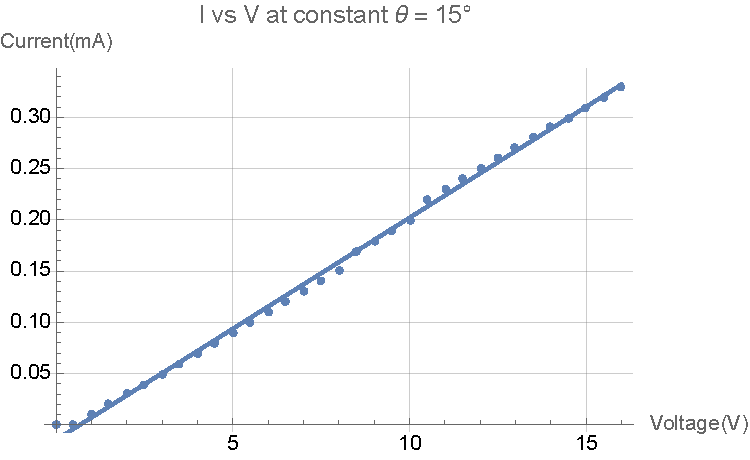
\includegraphics[width=1\textwidth]{graph1} % Include the figure
		\caption{}
	\end{figure}
	\subsection{Constant Flux at \(\theta = 45^{\circ}\) }
	\begin{center}
	\begin{tabular}{ | m{1cm} | m{3cm}| m{3cm} | } 
	\hline
	S.No & Voltage(V) & Current(mA) \\
	\hline
	1&0&0\\
	2&0.5&0\\
	3&1&0\\
	4&1.5&-0.01\\
	5&2&-0.02\\
	6&2.5&-0.03\\
	7&3&-0.03\\
	8&3.5&-0.04\\
	9&4&-0.05\\
	10&4.5&-0.06\\
	11&5&-0.06\\
	12&5.5&-0.07\\
	13&6&-0.08\\
	14&6.5&-0.09\\
	15&7&-0.1\\
	16&7.5&-0.1\\
	17&8&-0.11\\
	18&8.5&-0.12\\
	19&9&-0.13\\
	20&9.5&-0.14\\
	21&10&-0.14\\
	22&10.5&-0.15\\
	23&11&-0.16\\
	24&11.5&-0.17\\
	25&12&-0.18\\
	26&12.5&-0.18\\
	27&13&-0.19\\
	28&13.5&-0.2\\
	29&14&-0.2\\
	30&14.5&-0.21\\
	31&15&-0.22\\
	32&15.5&-0.23\\
	33&16&-0.24\\
	\hline

	\end{tabular}
	\end{center}
	Interpolated Function:- \(-0.0113191 + 0.0154679 x\) \\
	slope:- 0.0154679 
	\begin{figure}[H] % [H] forces the figure to be placed exactly where it appears in the text
		\centering % Horizontally center the figure
		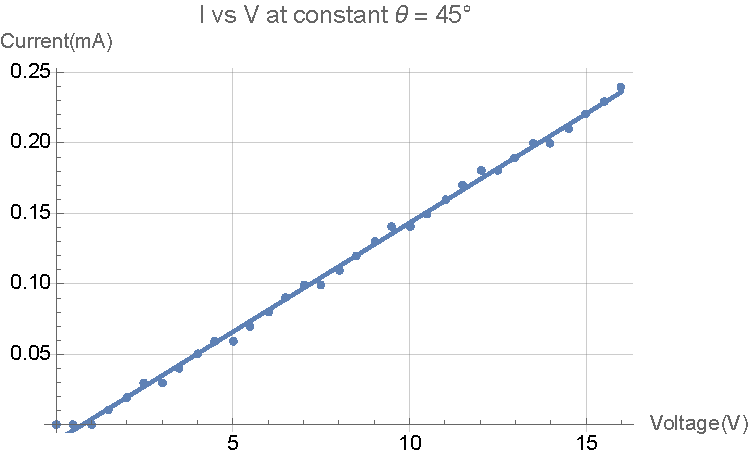
\includegraphics[width=1\textwidth]{graph2} % Include the figure
		\caption{}
	\end{figure}
	\subsection{Constant Flux at \(\theta = 75^{\circ}\) }
	\begin{center}
	\begin{tabular}{ | m{1cm} | m{3cm}| m{3cm} | } 
	\hline
	S.No & Voltage(V) & Current(mA) \\
	\hline
	1&0&0\\
	2&0.5&0\\
	3&1&-0.01\\
	4&1.5&-0.01\\
	5&2&-0.02\\
	6&2.5&-0.03\\
	7&3&-0.04\\
	8&3.5&-0.05\\
	9&4&-0.06\\
	10&4.5&-0.07\\
	11&5&-0.08\\
	12&5.5&-0.09\\
	13&6&-0.1\\
	14&6.5&-0.1\\
	15&7&-0.11\\
	16&7.5&-0.12\\
	17&8&-0.13\\
	18&8.5&-0.14\\
	19&9&-0.15\\
	20&9.5&-0.16\\
	21&10&-0.17\\
	22&10.5&-0.18\\
	23&11&-0.19\\
	24&11.5&-0.2\\
	25&12&-0.2\\
	26&12.5&-0.21\\
	27&13&-0.22\\
	28&13.5&-0.23\\
	29&14&-0.24\\
	30&14.5&-0.25\\
	31&15&-0.26\\
	32&15.5&-0.27\\
	33&16&-0.28\\
	\hline

	\end{tabular}
	\end{center}
	Interpolated Function:- \(-0.0115865 + 0.0180013 x\) \\
	slope:- 0.0180013 
	\begin{figure}[H] % [H] forces the figure to be placed exactly where it appears in the text
		\centering % Horizontally center the figure
		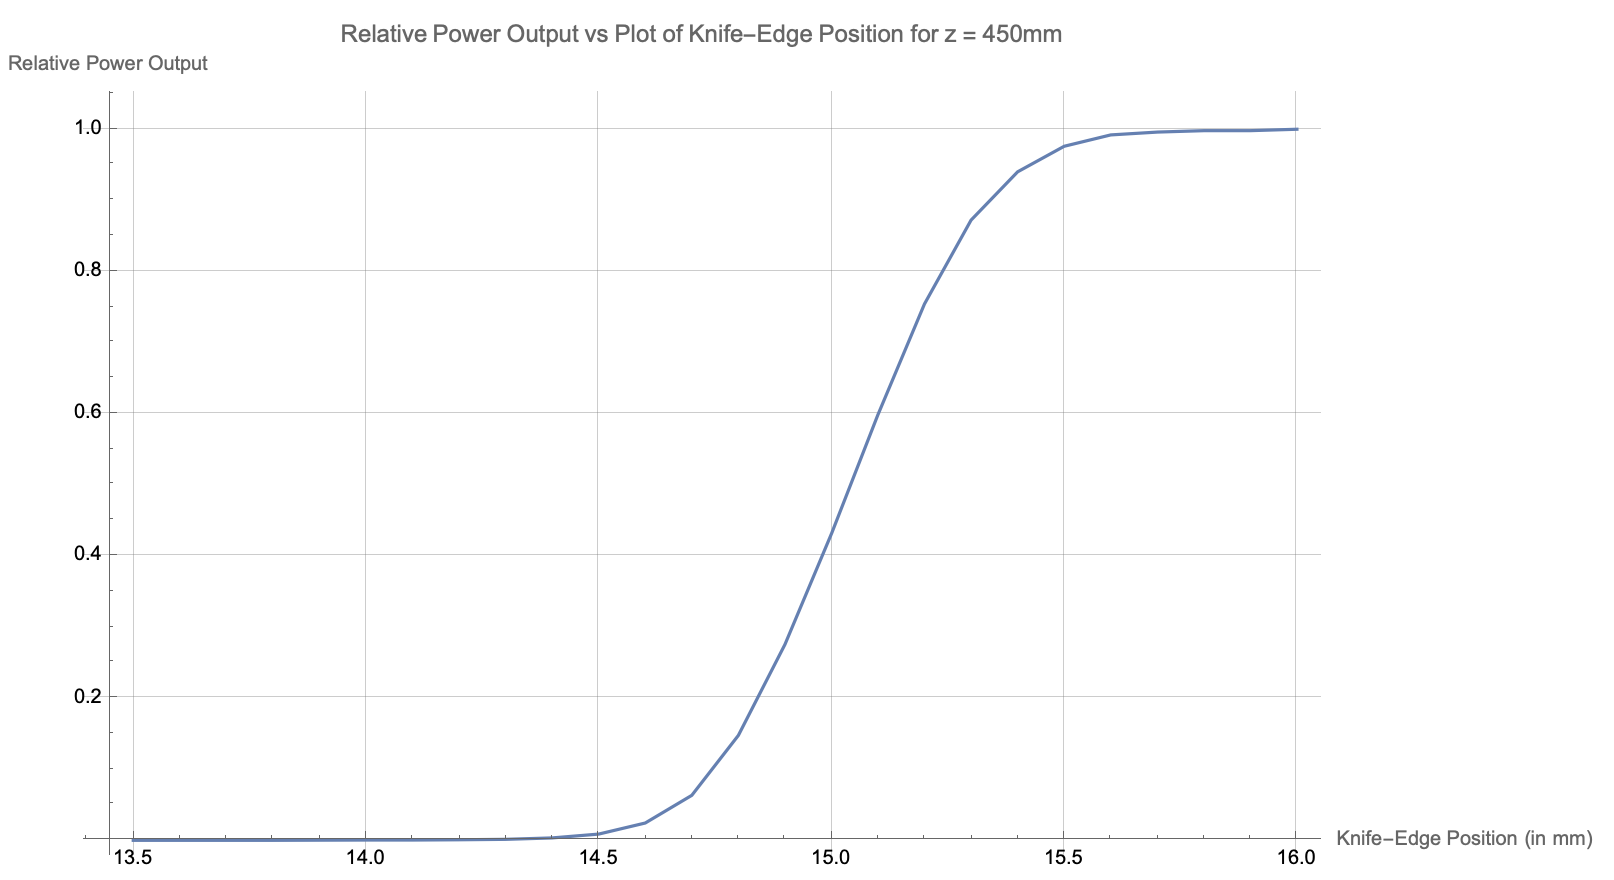
\includegraphics[width=1\textwidth]{graph3} % Include the figure
		\caption{}
	\end{figure}
	\subsection{Constant Voltage}
	\begin{center}
		\begin{tabular}{ | m{1cm} | m{1cm}| m{3cm} |m{3cm}  | m{3cm}|}
			\hline
			S.No&\(\theta\)  & V = 4V & V = 8V & V = 15V \\
			&&Current(mA)&Current(mA)&Current(mA)\\
			\hline

			0&0&-0.1&-0.1&-0.16\\
			1&10&-0.08&-0.08&-0.13\\
			2&20&-0.07&-0.07&-0.11\\
			3&30&-0.05&-0.05&-0.09\\
			4&40&-0.04&-0.03&-0.09\\
			5&50&-0.02&-0.02&-0.09\\
			6&60&-0.01&-0.02&-0.08\\
			7&70&-0.01&-0.02&-0.08\\
			8&80&-0.01&-0.04&-0.11\\
			9&90&-0.01&-0.05&-0.13\\
			10&100&-0.02&-0.06&-0.17\\
			11&110&-0.03&-0.08&-0.22\\
			12&120&-0.04&-0.1&-0.26\\
			13&130&-0.05&-0.11&-0.3\\
			14&140&-0.06&-0.13&-0.35\\
			15&150&-0.07&-0.15&-0.39\\
			16&160&-0.07&-0.16&-0.4\\
			17&170&-0.07&-0.15&-0.39\\
			18&180&-0.06&-0.13&-0.36\\
			\hline
		\end{tabular}
	\end{center}
	\begin{figure}[H] % [H] forces the figure to be placed exactly where it appears in the text
		\centering % Horizontally center the figure
		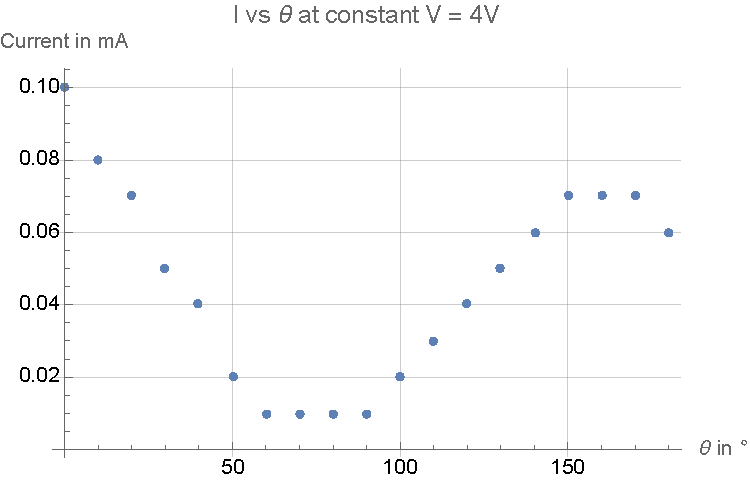
\includegraphics[width=1\textwidth]{graph4} % Include the figure
		\caption{}
	\end{figure}
	Minimum :- \(90^{\circ}\) 
	\begin{figure}[H] % [H] forces the figure to be placed exactly where it appears in the text
		\centering % Horizontally center the figure
		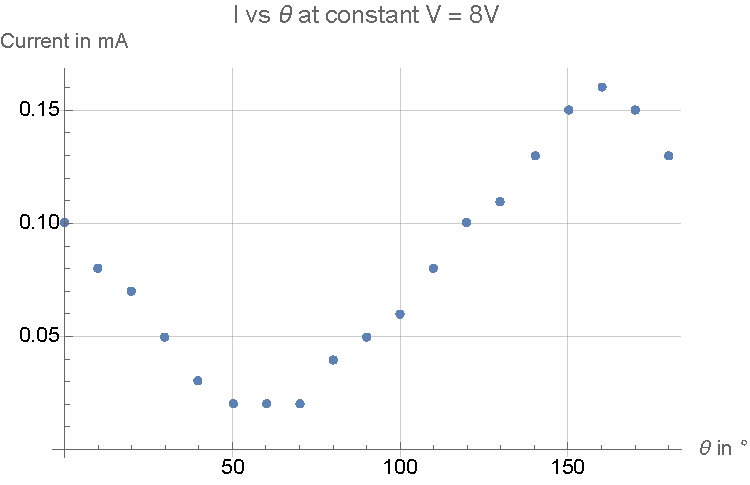
\includegraphics[width=1\textwidth]{graph5} % Include the figure
		\caption{}
	\end{figure}
	Minimum:- \(80^{\circ} \) 
	\begin{figure}[H] % [H] forces the figure to be placed exactly where it appears in the text
		\centering % Horizontally center the figure
		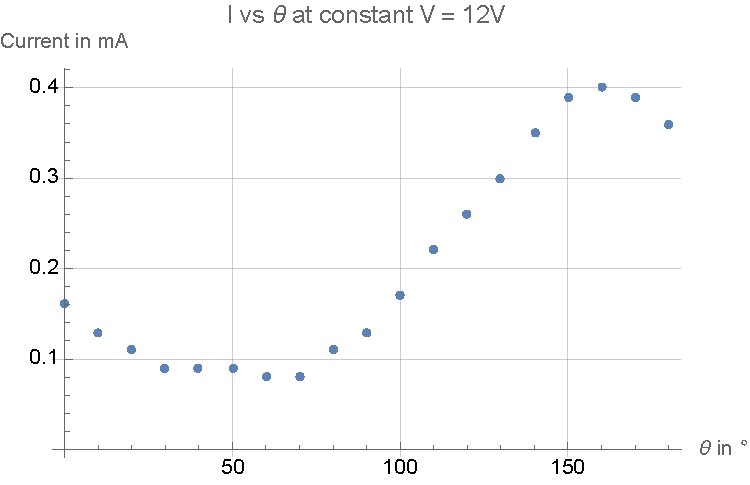
\includegraphics[width=1\textwidth]{graph6} % Include the figure
		\caption{}
	\end{figure}
	Minimum:- \(70^{\circ}\) 
	\section{Conclusion}
	Average of Slopes of I vs V graph = 0.0183712. This is the conductivity of the photo-resistor.
\end{document}
